\begin{slide}
\pagestyle{headings}
\sf
%\darkgreen
%
\bheader{{\normalsize \darkgreen Mini-exercise:} Find best data parametrisation}
%
\Large
The plots on the next two pages show  
$\chi^2$-fits of the same data distribution
with eight different 
parametrisations (polynomials of different orders).
%
Which parametrisation is the most reasonable one?
Try to judge using  the following three criteria:
\begin{enumerate}
\item 
optically, how well the curves fit the data
\item
 a reasonable parametrisation should lead to
$\chi^2/ndf \approx 1$.
\item
choose only a more complicated parametrisation if
a significant improvement of $\chi^2/ndf$ can be achieved
\end{enumerate}
$\rightarrow$ 
Try to find your personal favorite.
\end{slide}

\begin{slide}
\pagestyle{headings}
\sf
%
\bheader{{\normalsize \darkgreen Mini-exercise:} Find best data parametrisation}
\large
\begin{center}
\begin{figure}[h]
\unitlength1cm
  \begin{picture}(15,11.)
 \put(0.,0){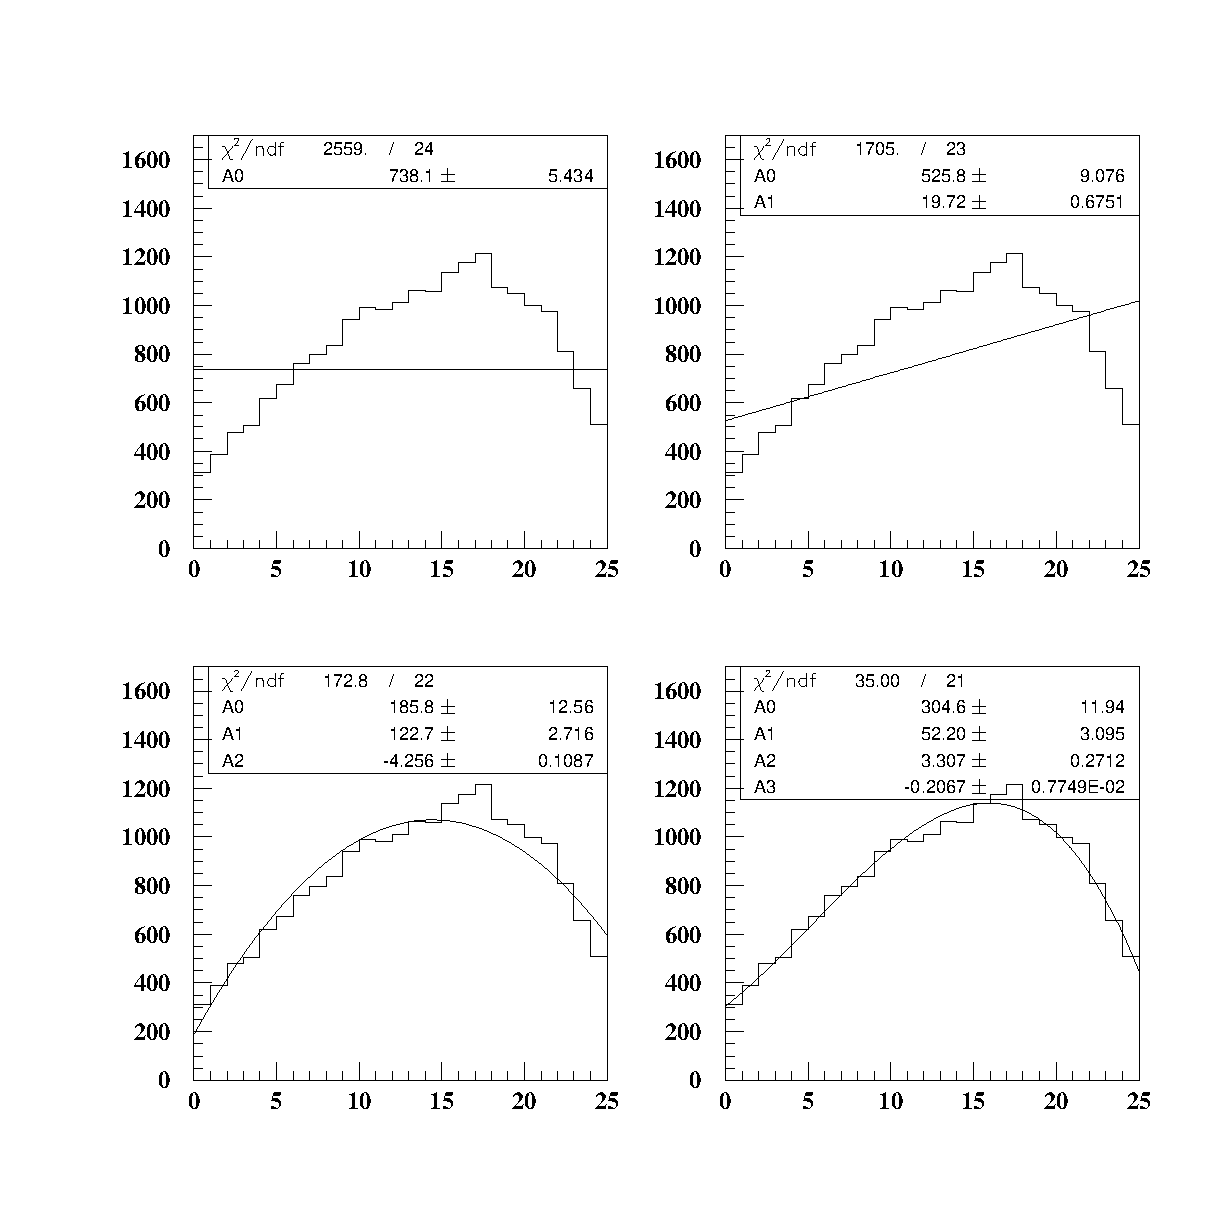
\epsfig{file=eps/p4_page1.eps,clip=,width=12.cm}}
\end{picture}
\end{figure}
\end{center}
\end{slide}

\begin{slide}
\pagestyle{headings}
\sf
%
\bheader{{\normalsize \darkgreen Mini-exercise:} Find best data parametrisation}

\large
\begin{center}
\begin{figure}[h]
\unitlength1cm
  \begin{picture}(15,11.)
 \put(0.,0){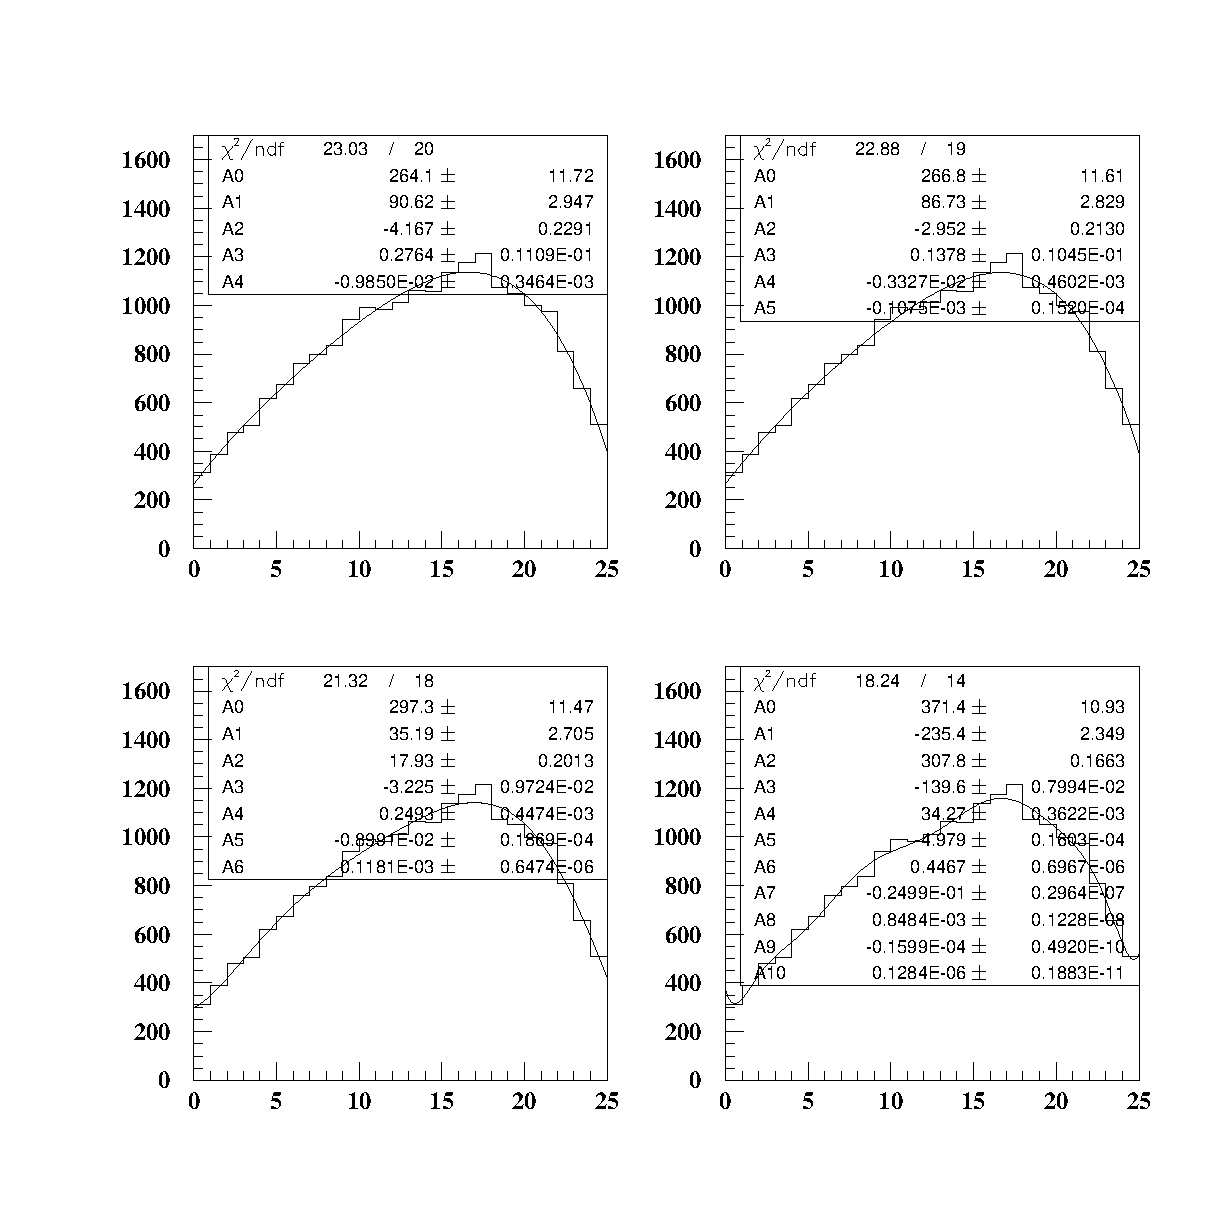
\epsfig{file=eps/p4_page2.eps,clip=,width=12.cm}}
\end{picture}
\end{figure}
\end{center}

\end{slide}
